\documentclass{article}
\pagenumbering{arabic}
\usepackage{graphicx,amsmath,amssymb,bm,tikz}
\usetikzlibrary{calc,patterns,decorations.pathmorphing,decorations.markings}
\usepackage{xfrac}
\usepackage[utf8]{inputenc}
\usepackage{hyperref}
% Format fref 
\usepackage[plain,english]{fancyref}
\usepackage[margin=1in]{geometry} 
\fancyrefaddcaptions{english}{\renewcommand*{\frefeqname}{Eq.}}
% Figure Packages
\usepackage[outercaption]{sidecap}
\usepackage[export]{adjustbox}
\usepackage{graphicx}
\usepackage{caption}
\usepackage{wrapfig}
\usepackage{float}
\usepackage{algorithm, algorithmic, amsfonts,amsmath,amssymb,amsthm, color,comment,enumitem, environ, fancyhdr,   graphicx, mathtools, wasysym}
\pagestyle{fancy}
\setlength{\headheight}{22.5pt}
\newenvironment{problem}[2][Problem]{\begin{trivlist}
\item[\hskip \labelsep {\bfseries #1}\hskip \labelsep {\bfseries #2.}]}{\end{trivlist}}
\newenvironment{sol}
    {\emph{Solution:}
    }
    {
    \qed
    }
\specialcomment{com}{ \color{blue} \textbf{Comment:} }{\color{black}} %for instructor comments while grading
\NewEnviron{probscore}{\marginpar{ \color{blue} \tiny Problem Score: \BODY \color{black} }}
%%%%%%%%%%%%%%%%%%%%%%%%%%%%%%%%%%%%%%%%%%%%%%%%%%%%%%%%%%%%%%%%%%%%%%%%%%%%%%%%%





%%%%%%%%%%%%%%%%%%%%%%%%%%%%%%%%%%%%%%%%%%%%%
%Fill in the appropriate information below
\lhead{Daniel Agramonte}  %replace with your name
\rhead{MCHE 6390 \\ Homework 5} %replace XYZ with the homework course number, semester (e.g. ``Spring 2019"), and assignment number.
%%%%%%%%%%%%%%%%%%%%%%%%%%%%%%%%%%%%%%%%%%%%%



% Table stuff
\usepackage{multirow}
%\usepackage{floatrow}
%	\floatsetup[table]{capposition=top}%puts table caption above
% Change \subsection title characteristics
    \usepackage[parfill]{parskip}   % forces parskip to not affect headings
    \usepackage{enumitem}           % used for editing itemize environment
    \usepackage{titlesec}
        \titleformat*{\section}{\Large\bfseries\titlerule\vspace{0.5em}}
% Quote blocks
    \usepackage{csquotes} % use environment 'displayquote'
% Misc document settings
    \title{\Huge MCHE 6390 Homework 5} \author{Daniel Agramonte} \date{12.02.20}
    \setlength{\parindent}{0pt}
    \setlength{\parskip}{1em}
    \setlist{nosep, itemsep=0pt, parsep=0pt}
% Misc vocab commands
    \newcommand{\msalg}{{\fontfamily{cmtt}\selectfont ms83}}
    \newcommand{\lsq}{\emph{lsqnonlin}}
    \newcommand{\msalge}{{\fontfamily{cmtt}\selectfont MCHE\_6500\_NIST\_POLY}}
%
% MATLAB packages
%
\usepackage[framed,numbered]{matlab-prettifier}
\usepackage{textcomp}
\usepackage{listings}
%
% Matrix Spacing
%
\makeatletter
\renewcommand*\env@matrix[1][\arraystretch]{%
  \edef\arraystretch{#1}%
  \hskip -\arraycolsep
  \let\@ifnextchar\new@ifnextchar
  \array{*\c@MaxMatrixCols c}}
\makeatother
%
\begin{document}
\maketitle

\begin{enumerate}
    \item 
    Work available attached at end
    \item 
    \begin{enumerate}
        \item 
        Normalized potential energy as a function of displacement
            \begin{figure}[H]
            \vspace{-10pt}
            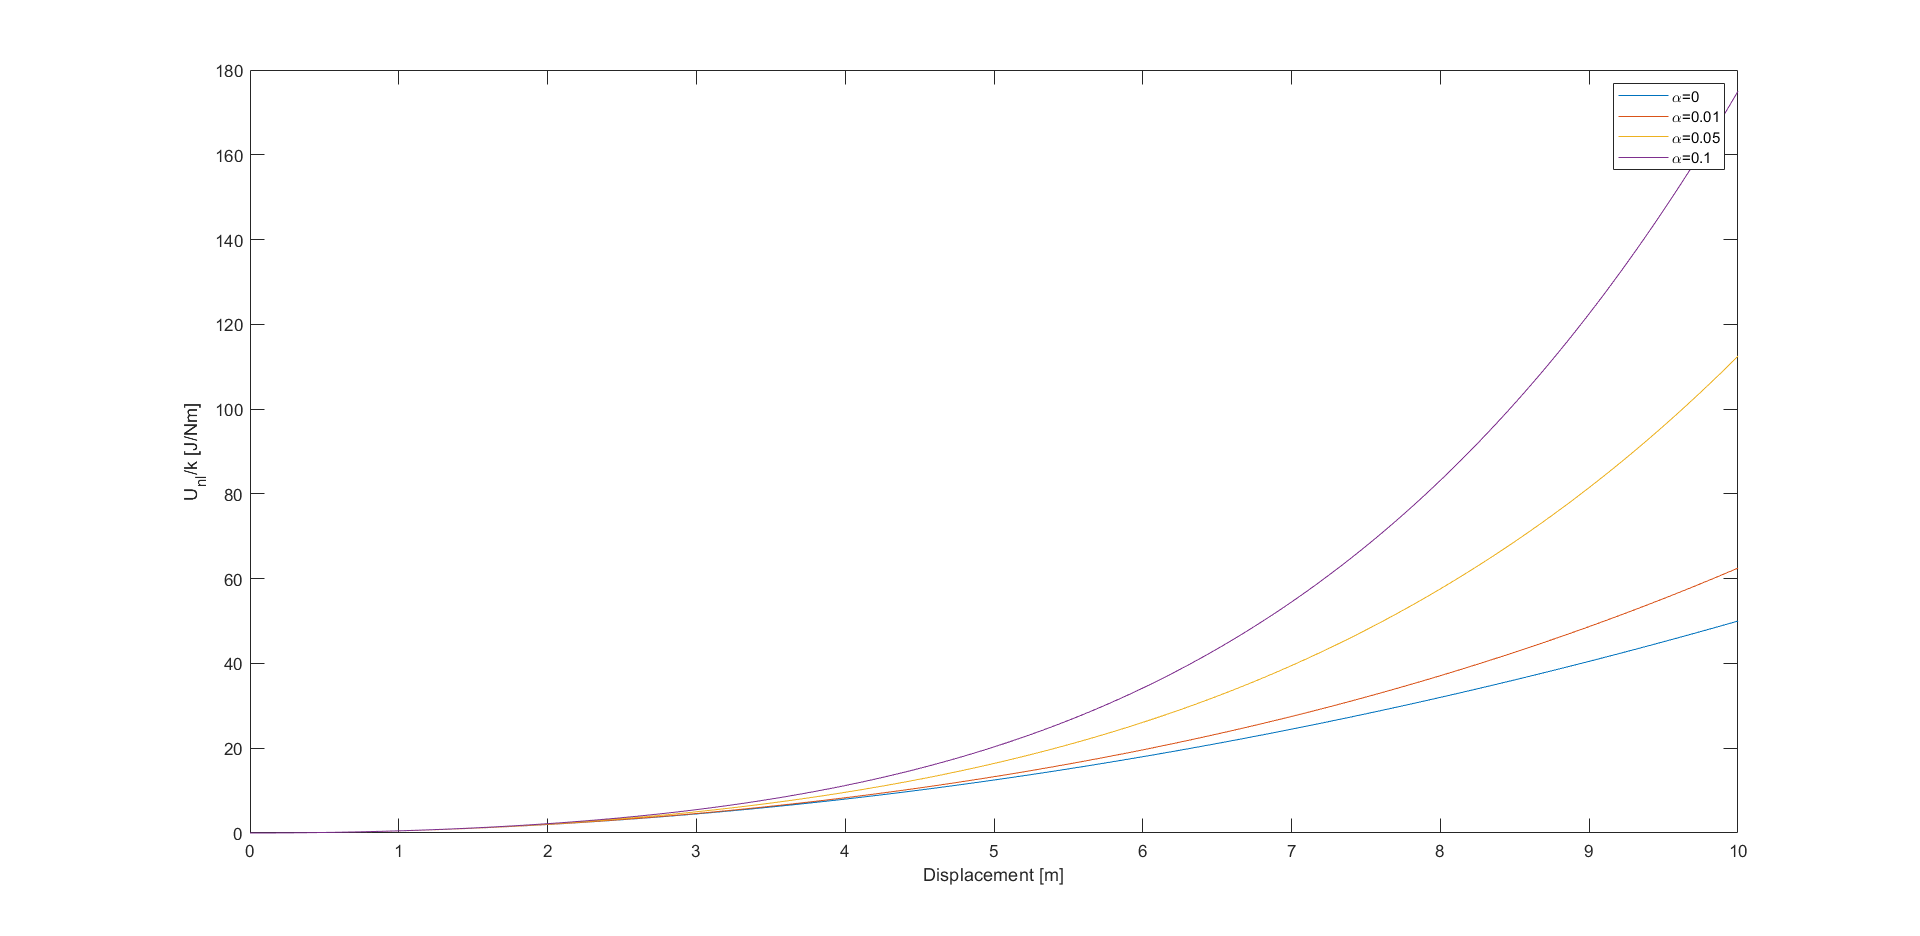
\includegraphics[width=\textwidth,left]{MCHE 6390/HW05/Figures/Figure_1_MCHE_6930_HW05.png}
            \label{fig:2a}
            \end{figure}
        \newpage
        \item
        Normalized force as a function of displacement
        \newline
            \begin{figure}[H]
            \vspace{-10pt}
            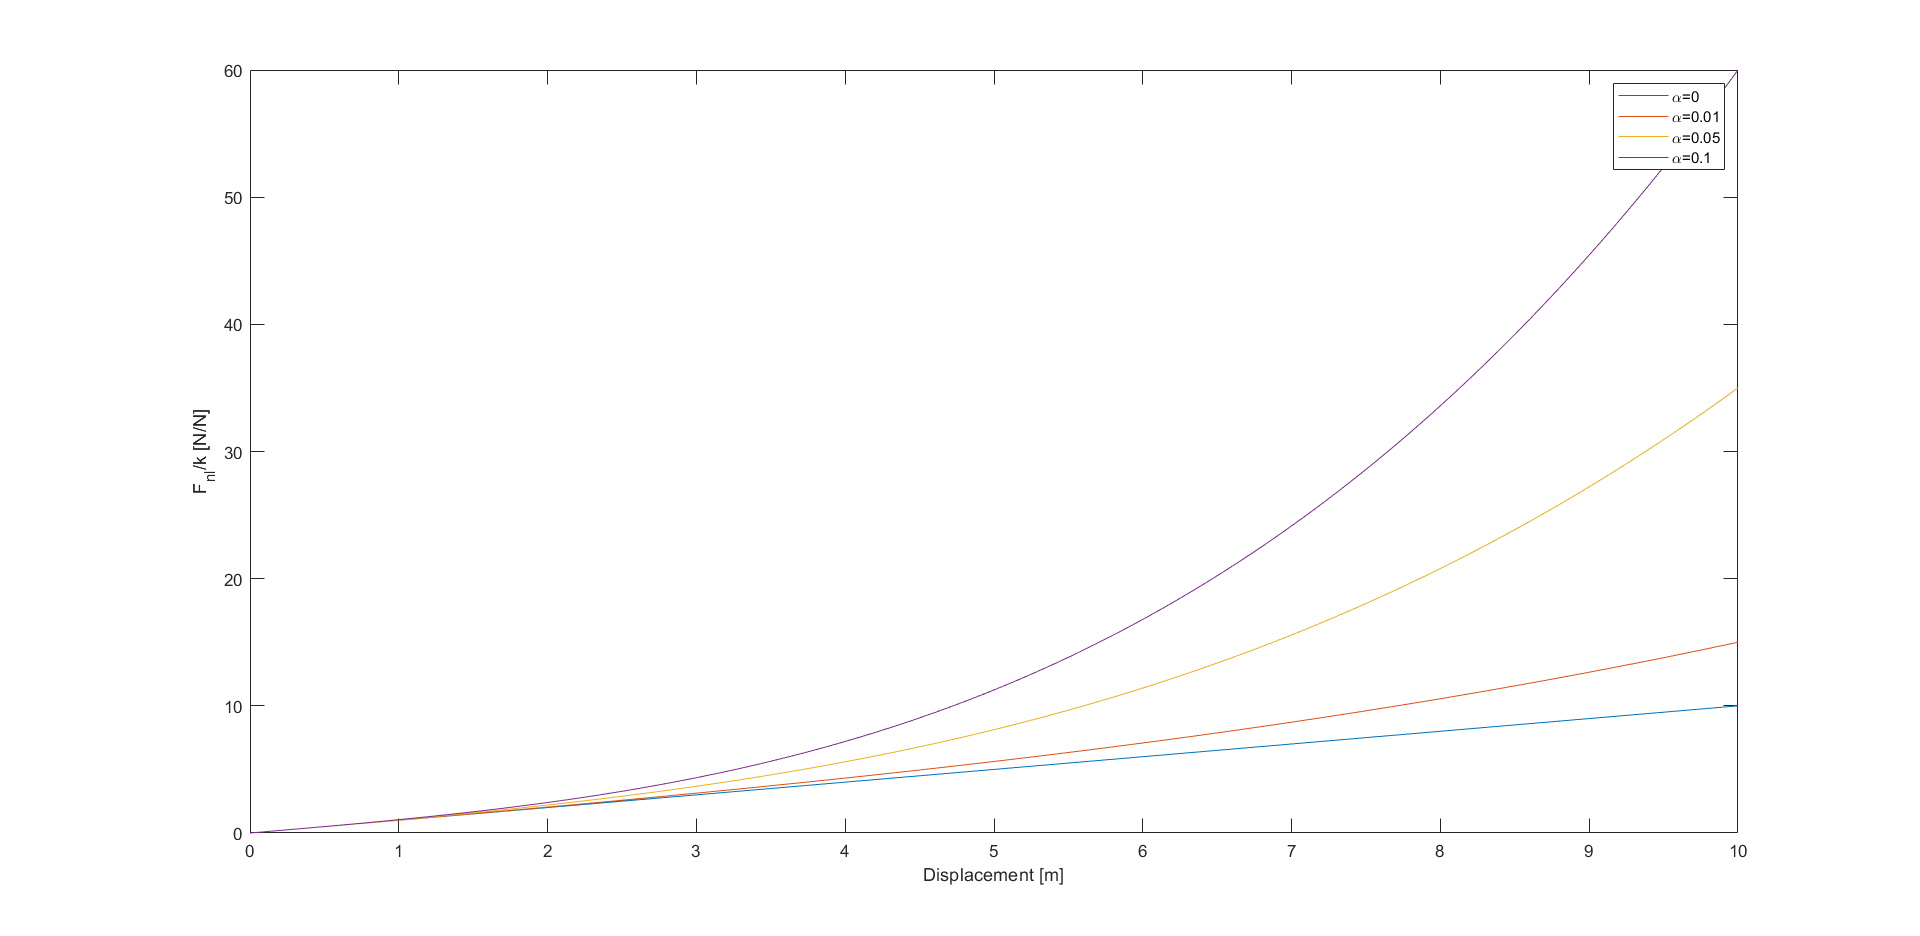
\includegraphics[width=\textwidth,left]{MCHE 6390/HW05/Figures/Figure_2_MCHE_6930_HW05.png}
            \label{fig:2b}
            \end{figure}
    MATLAB code I used to solve the entire problem
    \begin{lstlisting}[style=Matlab-editor]
    % Define delta x from 0 to 10
    x = linspace(0,10,1000);
    
    % Potential energy function
    U = @(a,x) 0.5*(x.^2+(a./4).*x.^4);
    
    % Force function
    F = @(a,x) x+(a./2).*x.^3;
    
    % Different values of alpha we care about
    a = [0,0.01,0.05,0.1];
    
    % Initialize and calculate potential energy and force
    Y_U = zeros(1000,4);
    Y_F = zeros(1000,4);
    
    for i = 1:4
        Y_U(:,i) = U(a(i),x);
        Y_F(:,i) = F(a(i),x);
    end
    
    figure(1)
    plot(x,Y_U)
    
    % Legend
    legend('\alpha=0','\alpha=0.01','\alpha=0.05','\alpha=0.1')
    
    % Axes
    xlabel('Displacement [m]')
    ylabel('U_{nl}/k [J/Nm]')
    
    figure(2)
    plot(x,Y_F)
    
    % Legend
    legend('\alpha=0','\alpha=0.01','\alpha=0.05','\alpha=0.1')
    
    % Axes
    xlabel('Displacement [m]')
    ylabel('F_{nl}/k [N/N]')
    \end{lstlisting}
        \item Please see hand written section at end for solution
        \item Please see hand written section at end for solution
        \end{enumerate}
    \item
    Please see hand written section at end for solution
    \item
    Please see hand written section at end for supplementary work.
    
    \begin{flalign*}
        \tau
        &=
        \begin{bmatrix}
        6.525  \\
        6.749 \\
        6.761 \\
        5.357 \\
        4.018 \\
        4.793
        \end{bmatrix}N \\
        \sigma/\sigma_{Y}
        &=
        \begin{bmatrix}
        0.0252  \\
        0.0449 \\
        0.0799 \\
        0.1424 \\
        0.2260 \\
        0.4027
        \end{bmatrix}.
    \end{flalign*}
    \newpage
    The following MATLAB code was additionally used to solve the problem
    
        \begin{lstlisting}[style=Matlab-editor]
        % Given in problem
        d = 0.0254*[0.042,0.032,0.024,0.016,0.011,0.009];
        f = [82.41,110,146.8,196,246.9,329.6];
        l = 25.5*0.0254;
        
        % Physical properties of steel
        E = 200*10^9;
        rho = 8050;
        S_y = 290*10^6;
        
        % Calculate tau
        tau = 0.25*(l^2)*(f.^2).*(d.^2)*rho;
        A = 0.25*pi*d.^2;
        P = tau./A;
        
        F = P/S_y;  

        \end{lstlisting}

    \item 
    We use the following MATLAB code to solve the problem
        \begin{lstlisting}[style=Matlab-editor]
        % Initialize error
        e = 1;
        
        % Starting number of terms
        n = 1;
        
        % x vector
        x = linspace(0,1,10000);
        
        while e>1/1000
        
        j = 1:n;
        
        % Initialize D
        D = zeros(n,1);
        
        for i = 1:n
            D(i) = d(i);
        end
        
        % Find error for each x
        E = (sum((D'.*ones(10000,1)).*sin(pi*j.*x'),2)-w_0(x))./w_0(x);
        
        % Find maximum error
        e = max(E(2:end-1));
        
        % Increment Process
        n = n+1;
        end
        
        plot(x,E)
        xlabel('Error [m]')
        ylabel('Position [m]')
        
        function V = d(n)
        V = 2*integral(@(x) w_0(x).*sin(n*pi*x), 0,1,'ArrayValued',true);
        end
        function V = w_0(x)
        V = zeros(length(x),1);
        for i =1:length(x)
            if x(i)<1/3
                V(i) = 3*x(i);
            elseif x(i)<0.5
                V(i) = 1;
            else
                V(i) = 2-2*x(i);
            end
        end
        
        end
        \end{lstlisting}
    From this we see that $n=114$.
    
    We now plot the error with respect to the displacement.
        \begin{figure}[H]
        \vspace{-10pt}
        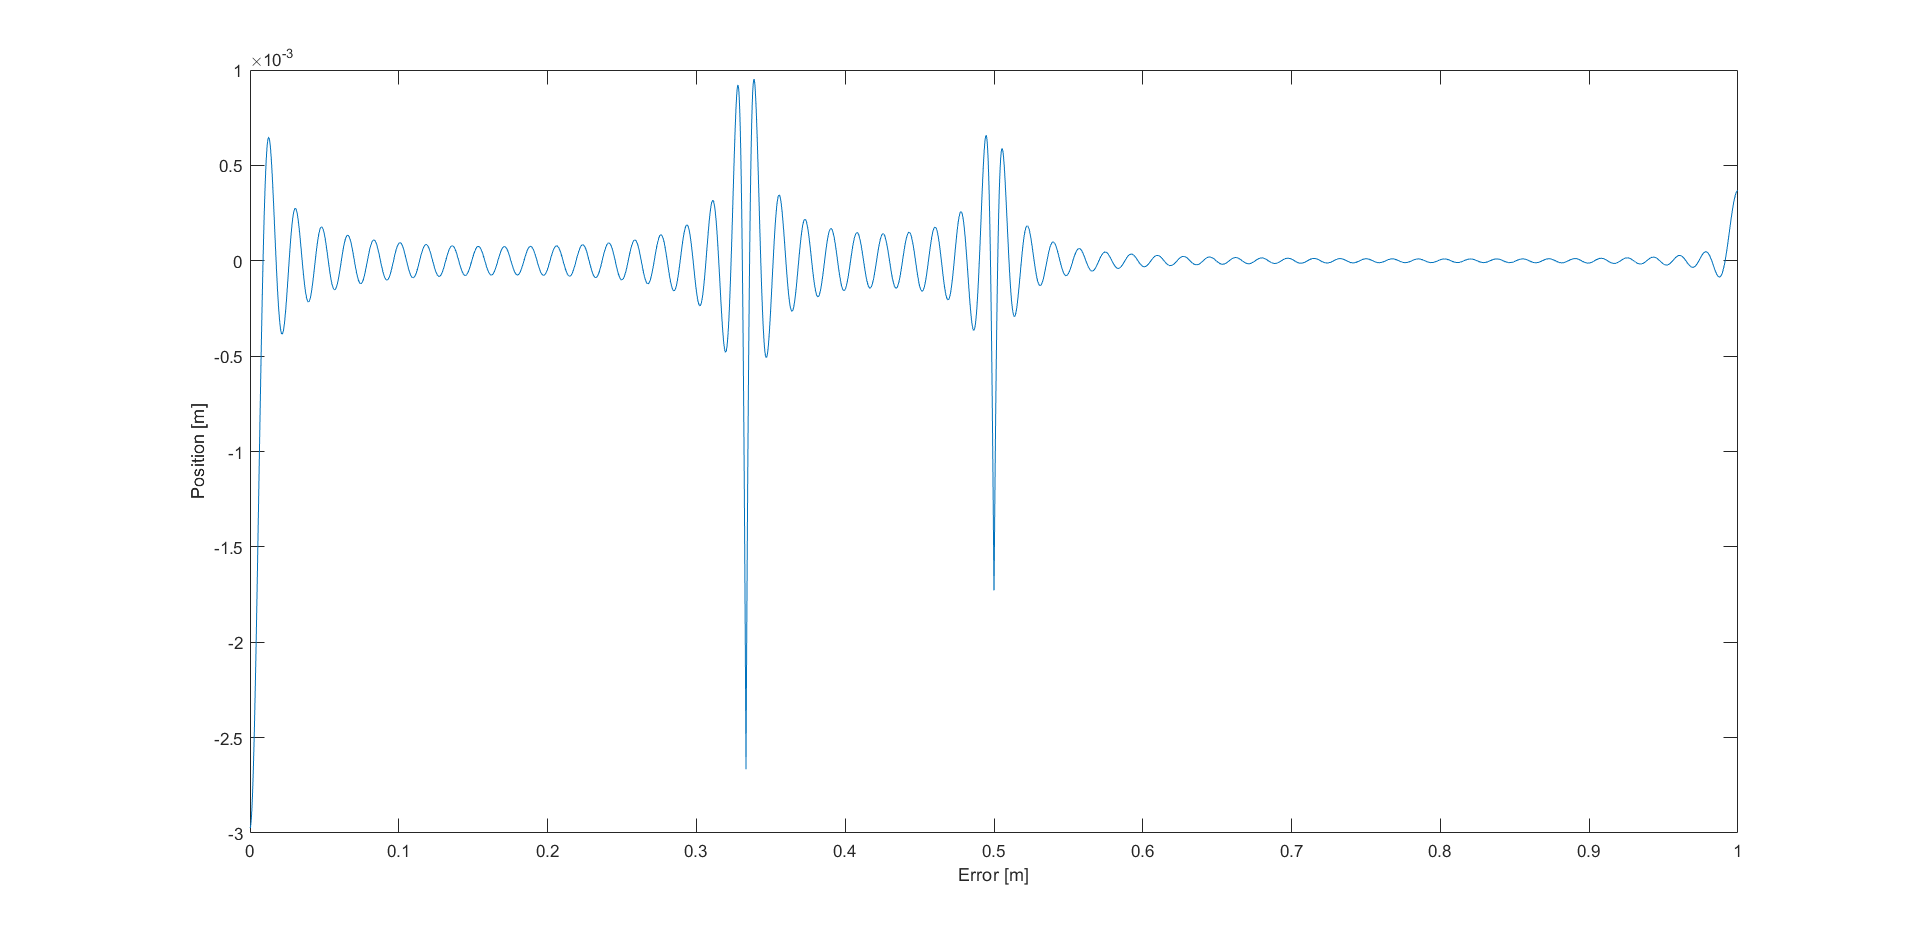
\includegraphics[width=\textwidth,left]{MCHE 6390/HW05/Figures/Figure_3_MCHE_6930_HW05.png}
        \label{fig:5}
        \end{figure}
    \item 
    \newpage
    See below MATLAB code which was used to solve the problem
        \begin{lstlisting}[style=Matlab-editor]
        % Composites
        
        rho_cm = (10^3)*[1.9,2.0,1.6,1.8,1.6,1.35];
        E_cm = (10^9)*[25,15.7,14.5,39.5,142,63.6];
        
        Comp_ws = sqrt(E_cm./rho_cm);
        Comp_ws_avg = mean(Comp_ws);
        
        % Metals
        
        rho_m = (10^3)*[7.15,7.7,2.7,2.7];
        E_m = (10^9)*[100,205,73,69];
        
        Metal_ws = sqrt(E_m./rho_m);
        Metal_ws_avg = mean(Metal_ws);
        
        % Ceramics
        
        rho_c = (10^3)*[3.8,3.6];
        E_c = (10^9)*[350,205];
        
        Cer_ws = sqrt(E_c./rho_c);
        Cer_ws_avg = mean(Cer_ws);
        
        % Plastics
        
        rho_p = (10^3)*[1.15,1.15,1.07,1.25,1.35];
        E_p = (10^9)*[2.8,0.89,1.4,3.5,3.0];
        
        Plas_ws = sqrt(E_p./rho_p);
        Plas_ws_avg = mean(Plas_ws);
        \end{lstlisting}
    \begin{flalign*}
        c_{ceramics}
        &=
        \begin{bmatrix}
        9597  \\
        7546 \\
        \end{bmatrix}\text{m/s} \\
        c_{ceramics,avg} &= 8572\text{ m/s} \\
        c_{composites}
        &=
        \begin{bmatrix}
        3627  \\
        2802 \\
        3010 \\
        4685 \\
        9421 \\
        6864
        \end{bmatrix}\text{ m/s} \\
        c_{composites,avg} &= 5068\text{m/s} \\
        c_{metal}
        &=
        \begin{bmatrix}
        3840  \\
        5160 \\
        5055 \\
        \end{bmatrix}\text{m/s} \\
        c_{metal,avg} &= 4789\text{ m/s} \\
        c_{plastic}
        &=
        \begin{bmatrix}
        1560  \\
        880 \\
        1144 \\
        1673 \\
        1491
        \end{bmatrix}\text{m/s} \\
        c_{plastic,avg} &= 1350\text{ m/s}
    \end{flalign*}
    Note that the ordering of the wave speeds is the same as on Engineering Toolbox.
\item
    \begin{flalign*}
        \ell
        &=
        \begin{bmatrix}
        0.0633  \\
        0.0575 \\
        0.0527 \\
        0.0487 \\
        0.0452 \\
        0.0396 \\
        0.0372 \\
        0.0352 \\
        0.0333 \\
        0.0316
        \end{bmatrix}\text{m.} \\
    \end{flalign*}
    The following MATLAB code was used
        \begin{lstlisting}[style=Matlab-editor]
            % Frequencies of interest
            f = 10000:1000:20000;
            
            % Note that we only are considering the fundamental modes of the bar, hence
            % the dropping out of the 
            l = sqrt((50*10^9)/7800)./(4*f);
        \end{lstlisting}
    \item
    First 10 natural frequencies
    \begin{flalign*}
        f_{n}
        &=
        \begin{bmatrix}
        607.2  \\
        1349.4 \\
        2147.6 \\
        2963.7 \\
        3786.9 \\
        4613.7 \\
        5442.4 \\
        6272.4 \\
        7103.1 \\
        7934.4
        \end{bmatrix}\text{Hz.} \\
    \end{flalign*}
        \begin{lstlisting}[style=Matlab-editor]
            % Transcendental Equation
            tr_eq = @(sl) tan(sl)+0.5*sl;
            
            x = linspace(0,20,100000);
            
            % Initialize zeros vector
            z = zeros(10,1);
            
            for i = 1:length(z)
                z(i) = fzero(tr_eq,[1.58+(i-1)*pi,4+(i-1)*pi]);
            end
            
            f = ((z/3)*sqrt((200*10^9)/8000))/(2*pi);
        \end{lstlisting}
\end{enumerate}

\end{document}
